\normaltrue
\correctionfalse

%\UPSTIidClasse{11} % 11 sup, 12 spé
%\newcommand{\UPSTIidClasse}{11}

\exer{Mouvement RR  $\star$ \label{C1:05:04}}
\setcounter{numques}{0}
\UPSTIcompetence[2]{B2-14}
\UPSTIcompetence[2]{B2-15}
\UPSTIcompetence[2]{C1-05}
\index{Compétence B2-14}
\index{Compétence B2-15}
\index{Compétence C1-05}
\index{Torseur des actions mécaniques transmissibles}
\index{Torseur d’une action mécanique extérieure}
\index{Principe fondamental de la statique}
\index{PFS}
\index{Mécanisme à 2 rotations}
\ifcorrection
\else
\textbf{Pas de corrigé pour cet exercice.}
\fi

\ifprof
\else
Soit le mécanisme suivant. On a $\vect{AB}=R\vect{i_1}$ avec $R=\SI{20}{mm}$ et  
$\vect{BC}=L\vect{i_2}$ avec $L=\SI{15}{mm}$. De plus :
\begin{itemize}
\item $G_1$ désigne le centre d'inertie de \textbf{1} et $\vect{AG_1}=\dfrac{1}{2}R\vect{i_1}$, on note $m_1$ la masse de \textbf{1}; %et $\inertie{G_1}{1}=\matinertie{A_1}{B_1}{C_1}{0}{0}{0}{\bas{1}}$; 
\item $G_2$ désigne le centre d'inertie de \textbf{2} et $\vect{BG_2}=\dfrac{1}{2}L\vect{i_2}$, on note $m_2$ la masse de \textbf{2}.% et $\inertie{G_2}{2}=\matinertie{A_2}{B_2}{C_2}{0}{0}{0}{\bas{2}}$.
\end{itemize}

Un moteur électrique positionné entre \textbf{0} et \textbf{1} permet de maintenir \textbf{1} en équilibre.
Un moteur électrique positionné entre \textbf{1} et \textbf{2} permet de maintenir \textbf{2} en équilibre.

L'accélération de la pesanteur est donnée par $\vect{g}=-g\vect{j_0}$.

\begin{center}
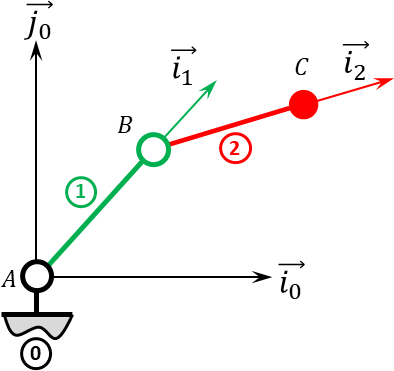
\includegraphics[width=\linewidth]{04_RR_01}
\end{center}
\fi

\question{Réaliser le graphe d'analyse en faisant apparaître l'ensemble des actions mécaniques.}
\ifprof
\else
\fi

\question{Donner le torseur de chacune des actions mécaniques.}
\ifprof
\else
\fi

\question{Simplifier les torseurs dans l'hypothèse des problèmes plans.}
\ifprof
\else
\fi

\question{Proposer une démarche permettant de déterminer les couples que doivent développer chacun des moteurs  pour maintenir le mécanisme en équilibre.}
\ifprof
\else
\fi



\ifprof
\else
\begin{flushright}
\footnotesize{Corrigé  voir \ref{C1:05:04}.}
\end{flushright}%
\fi